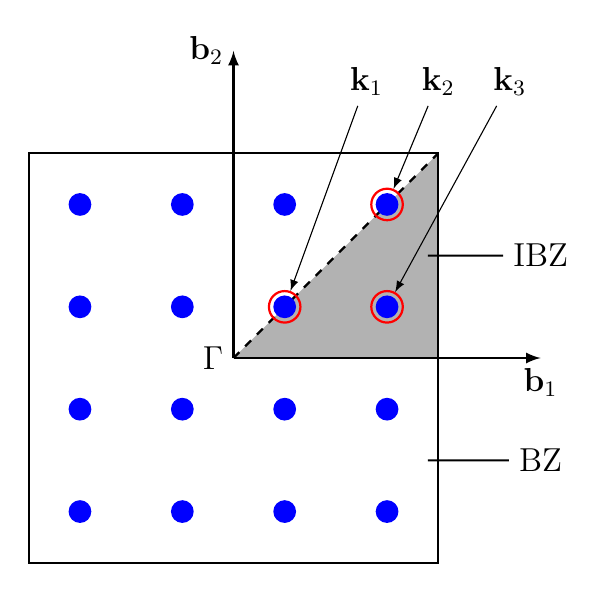
\begin{tikzpicture}[scale=1.3, font=\large, >=latex, auto, thick, 
kcircle/.style={draw, circle, color=red, minimum size = 0.4cm} 
] 
    % Reciprocal axes 
    \draw [->] (0, 0) node [left] {$\Gamma$} -- (3, 0) node [below] 
{$\mathbf{b}_1$}; 
    \draw [->] (0, 0) -- (0, 3) node [left] {$\mathbf{b}_2$}; 
     
    % Brillouin zone 
    \draw (-2, -2) rectangle (2, 2); 
    \draw [dashed] (0, 0) -- (2, 2); 
    \path [fill=black, fill opacity=0.3] (0, 0) -- (2, 2) -- (2, 0) -- cycle; 
     
    % k-points 
    \foreach \x in {-1.5, -0.5, ..., 1.5} 
        \foreach \y in {-1.5, -0.5, ..., 1.5} 
            \draw[fill=blue, color=blue] (\x,\y) circle (0.1cm); 
     
    \node (k1) at (0.5, 0.5) [kcircle] {}; 
    \node (k2) at (1.5, 1.5) [kcircle] {}; 
    \node (k3) at (1.5, 0.5) [kcircle] {}; 
     
    % Annotation 
    \node (k1_anno) at (1.3, 2.7) {$\mathbf{k}_1$}; 
    \draw [->, thin] (k1_anno)  -- (k1); 
    \node (k2_anno) at (2, 2.7) {$\mathbf{k}_2$}; 
    \draw [->, thin] (k2_anno)  -- (k2); 
    \node (k3_anno) at (2.7, 2.7) {$\mathbf{k}_3$}; 
    \draw [->, thin] (k3_anno)  -- (k3); 
     
    \node (bz) at (3, -1) {BZ}; 
    \draw (1.9, -1) -- (bz); 
    \node (ibz) at (3, 1) {IBZ}; 
    \draw (1.9, 1) -- (ibz); 
     
\end{tikzpicture} 
